\documentclass[a4paper,10pt]{article}
\usepackage[margin=1in]{geometry}
\usepackage{polski}
\usepackage[T1]{fontenc}
\usepackage[utf8]{inputenc}
\usepackage[unicode]{hyperref}
\usepackage{amssymb}
\usepackage{xifthen}
\usepackage[fleqn]{amsmath}
\usepackage{todonotes}
\usepackage{graphicx}
\usepackage{float}
\usepackage{fullpage}
\usepackage{epstopdf}
\usepackage{multirow}
\usepackage{subfig}
\usepackage{booktabs}
\usepackage[europeanresistors,americaninductors]{circuitikz}
\usetikzlibrary{patterns}
\newcommand{\withtodo}{0}

\def\arraystretch{1.2}

\begin{document}

\begin{table}
  \centering
  \def\arraystretch{1.5}
    \begin{tabular}{|c|c|c|c|c|} \hline
    \multicolumn{5}{|c|}{Wstęp do Fizyki Ciała Stałego}\\
		\multicolumn{5}{|c|}{Zadanie Projektowe} \\\hline
    Imię i nazwisko	&	nr albumu	&	grupa	&	data oddania	&	nr zestawu: 1	\\\hline
				Paulina			&		284494	&		R3	&		18 I 2018		&	nr zadan:  \\
				Marikin			&						&				&								&	1,3,5 \\\hline
  \end{tabular}
\end{table}


\section{Zadanie 1: Analiza Termiczna}

\begin{figure}[H]
	\centering
		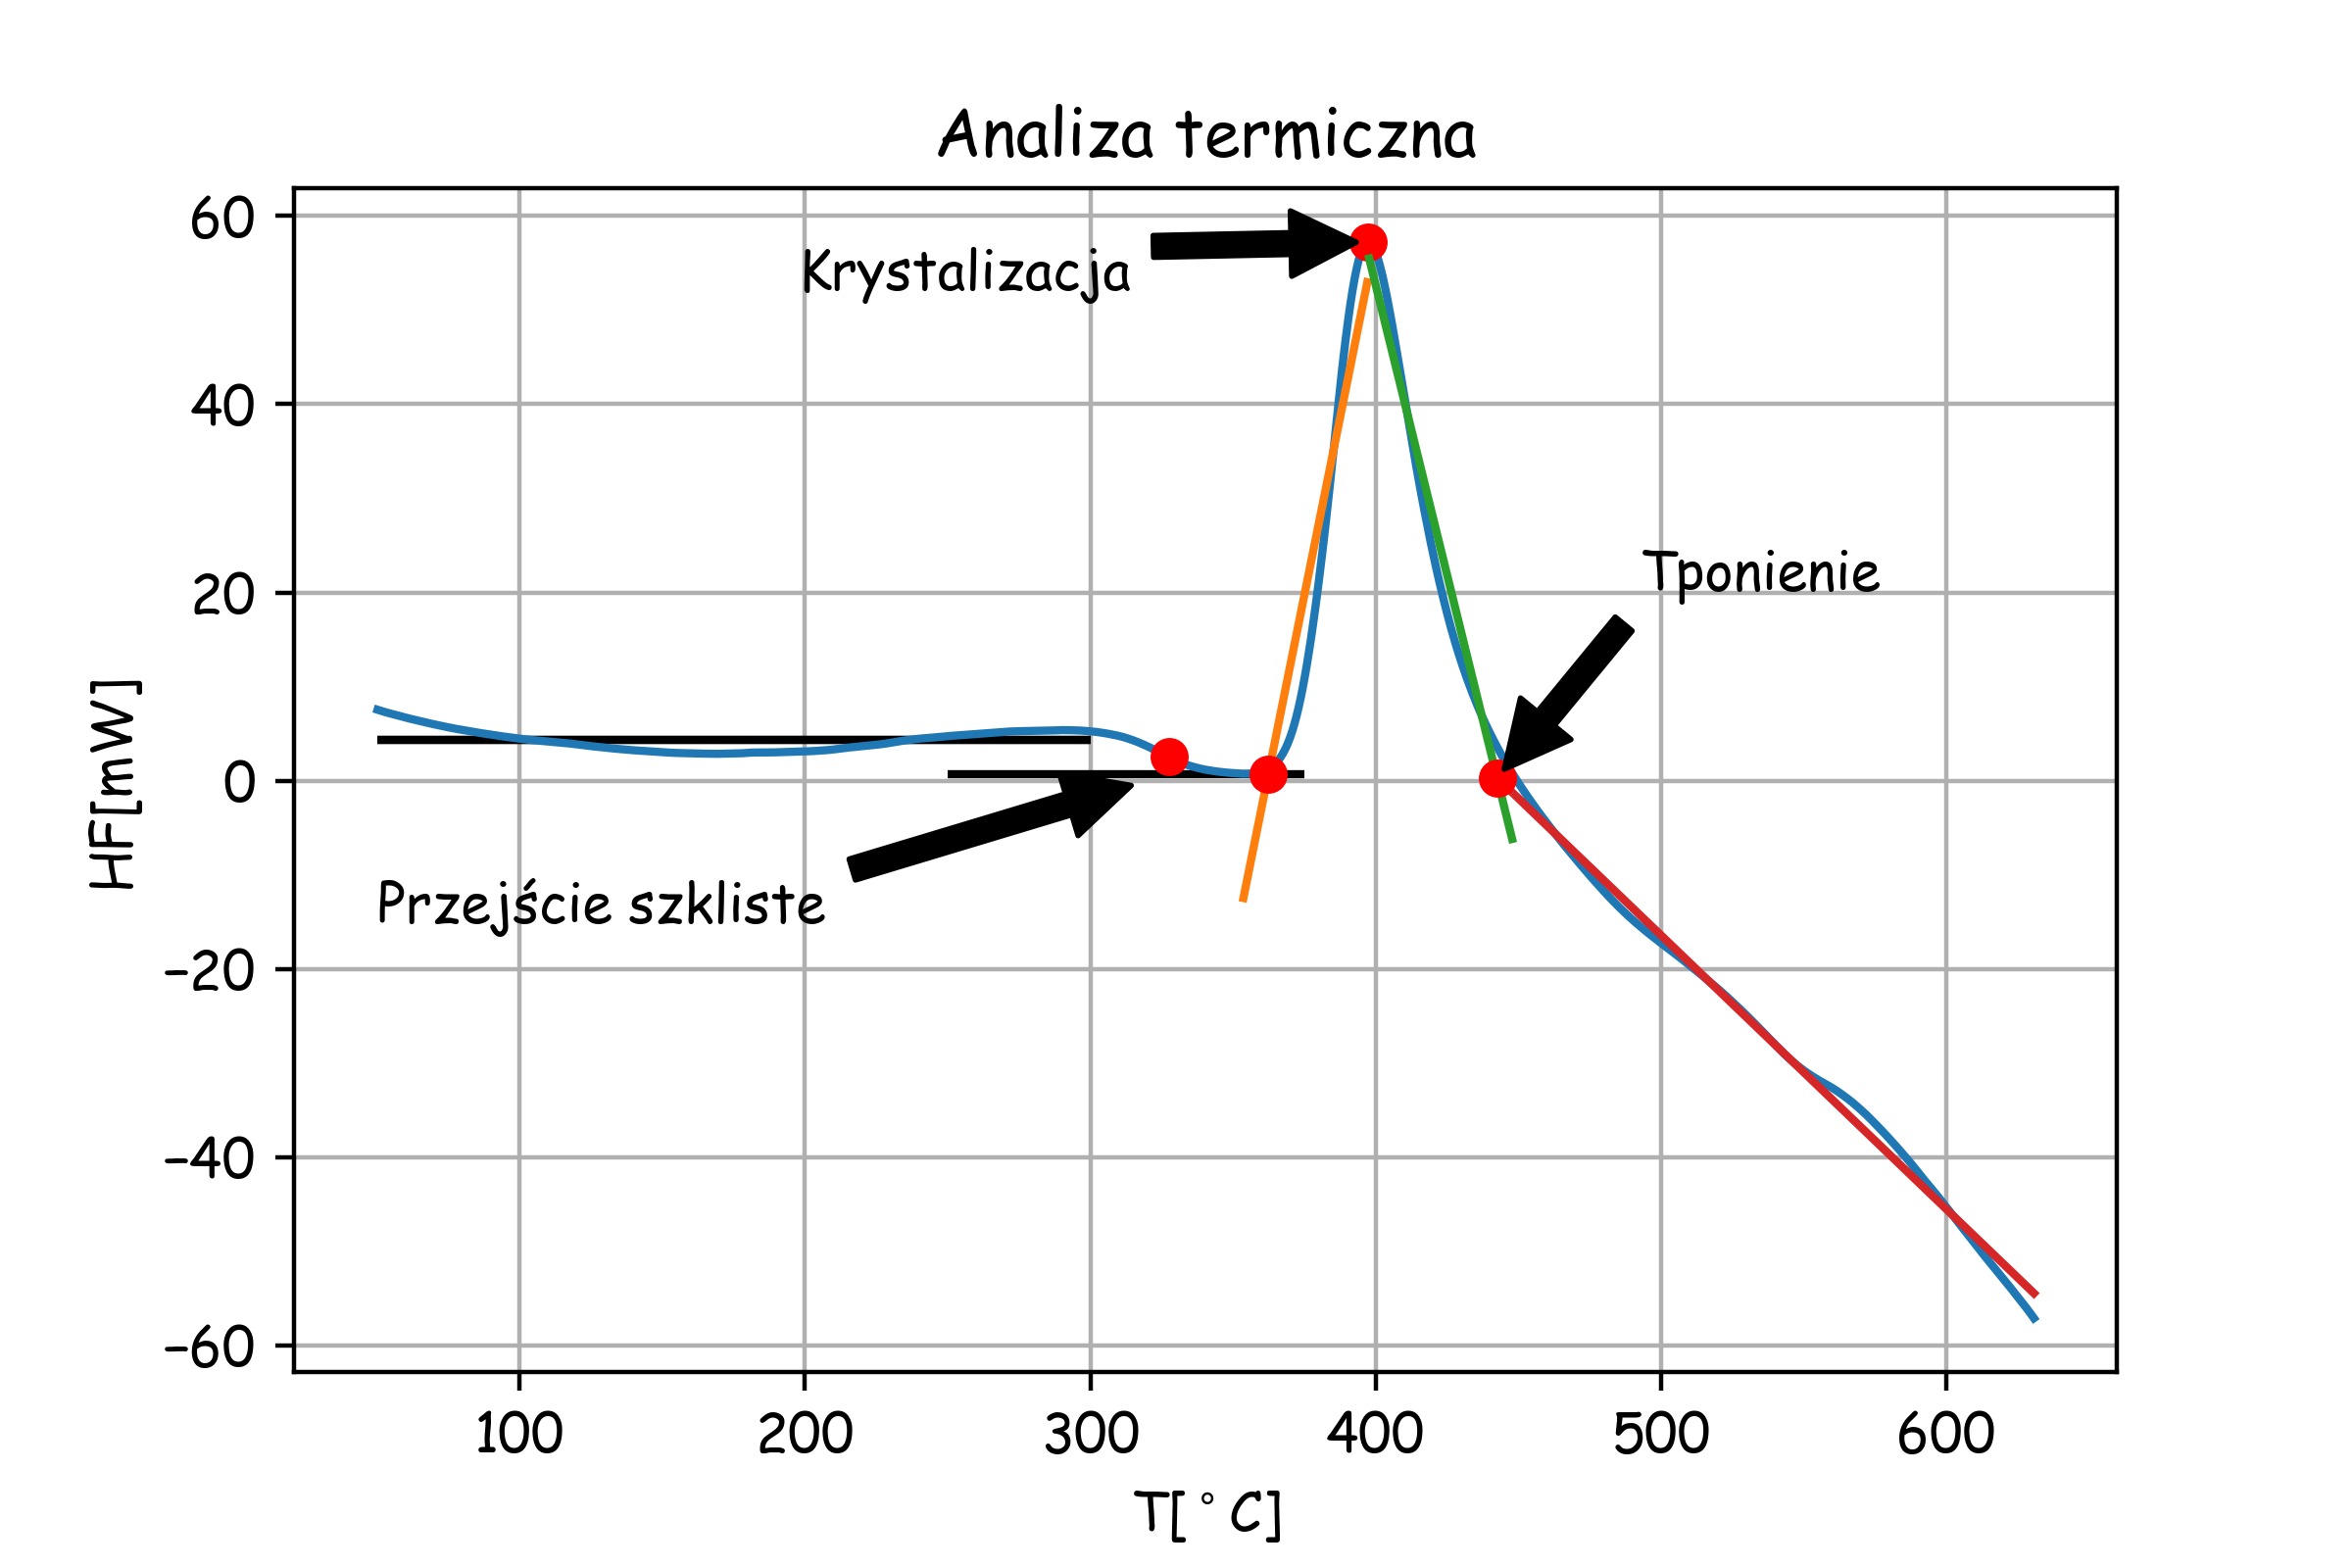
\includegraphics[width=\textwidth]{../Analiza_termiczna.png}
\end{figure}

\subsection{Przejście szkliste}
Temperatura: 327.571$^\circ$C \\
Wyznaczanie:
\begin{itemize}
	\item Do początkowej cześci wykresu przed rozpoczęciem przejścia (do około 300 $^\circ$C) dopasowałam poziomą prostą (prosta fioletowa).
	\item Dla maksymalnego spadku temperatury po przejściu wyznaczyłam HF i na jego wysokości wyrysowałam poziomą prostą (prosta niebieska).
	\item Z powyższych wartości wyliczyłam średnią wartość HF.
	\item Pomiar o HF najbardziej zbliżonym do danej średniej uznałam za środek przejścia szklistego. Temperaturę w tym pomiarze uznałam za temperaturę przejścia szklistego.
\end{itemize}

\subsection{Krystalizacja}
Temperatura początku krystalizacji: 362.439 $^\circ$C \\
Wyznaczanie: \\
Do pierwszej części krystalizacji (rosnące HF) dopasowałam prostą (pomarańczowa prosta). Następnie wyliczyłam punkt jej przecięcia z uprzednio wyrysowaną prostą niebieską. Temperatura tego punktu uznałam za temperaturę początku krystalizacji.
Temperatura krystalizacji: 397.421 $^\circ$C \\
Wyznaczanie: \\
Jest to temperatura pomiaru o najwyższym HF w piku krystalizacji.

\subsection{Topnienie}
Temperatura: 442.567$^\circ$C \\
Wyznaczanie: \\
Jest to temperatura punktu przecięcie prostej dopasowanej do drugiej części piku krystalizacji (dla malejącego HF) z prostą dopasowaną do dalszego spadku HF (kolejno proste zielona i błękitna).
 
\section{Zadanie 3: Dyfraktometria Rentgenowska}
Położenie maksimów wyznaczyłam dla manganu: 
\begin{itemize}
	\item Stała sieciowa: 8.91 \AA
\item Struktura: BCC
\item Położenia atomów w komórce elementarnej: [0,0,0] i [$\frac{1}{2}$,$\frac{1}{2}$,$\frac{1}{2}$]
\end{itemize}
Na mangan świecono falą o długości $\lambda = 1.66$ \AA. 
Dla struktury BCC, będącej wariacją struktury sześciennej $d=\frac{a}{\sqrt{h^2 +k^2 + l^2}}$. Z twierdzenia Wullfa-Braggów wiadomo że $2 d \sin{\theta} =n\lambda$, więc $2 \theta = \arcsin{\frac{n\lambda} {2 d}} $, gdzie n to rząd ugięcia. Czynnik struktury F ma postać $F=\sum\limits_j f_j * e^{2 \pi i(h*x_j+k*y_j+l*z_j)} $ co dla manganu daje $F=f *( 1+e^{i\pi (h+k+l)}) $ \\
\begin{tabular}{|cccccc|}
\hline
\hline
  h &  k &  l &  $d_{hkl}[\AA]$ &  $2\theta[^\circ C]$ &$F_{hkl}[*f]$ \\
\hline
\hline
  0 &  1 &  2 &     3.984673 &            24.045275 &            0 \\\hline
  0 &  1 &  3 &     2.817589 &            34.264475 &            2 \\\hline
  0 &  1 &  4 &     2.160992 &            45.173621 &            0 \\\hline
  0 &  1 &  5 &     1.747395 &            56.717768 &            2 \\\hline
  0 &  1 &  6 &     1.464795 &            69.031422 &            0 \\\hline
  0 &  1 &  7 &     1.260064 &            82.401080 &            2 \\\hline
  0 &  2 &  3 &     2.471189 &            39.250982 &            0 \\\hline
  0 &  2 &  4 &     1.992337 &            49.239764 &            2 \\\hline
  0 &  2 &  5 &     1.654545 &            60.218228 &            0 \\\hline
  0 &  2 &  6 &     1.408795 &            72.194292 &            2 \\\hline
  0 &  2 &  7 &     1.223883 &            85.401550 &            0 \\\hline
  0 &  3 &  4 &     1.782000 &            55.519978 &            0 \\\hline
  0 &  3 &  5 &     1.528052 &            65.800088 &            2 \\\hline
  0 &  3 &  6 &     1.328224 &            77.348877 &            0 \\\hline
  0 &  4 &  5 &     1.391508 &            73.235720 &            0 \\\hline
  0 &  4 &  6 &     1.235595 &            84.403206 &            2 \\\hline
  1 &  2 &  3 &     2.381298 &            40.797238 &            2 \\\hline
  1 &  2 &  4 &     1.944321 &            50.539965 &            0 \\\hline
  1 &  2 &  5 &     1.626736 &            61.357524 &            2 \\\hline
  1 &  2 &  6 &     1.391508 &            73.235720 &            0 \\\hline
  1 &  2 &  7 &     1.212497 &            86.398496 &            2 \\\hline
  1 &  3 &  4 &     1.747395 &            56.717768 &            2 \\\hline
  1 &  3 &  5 &     1.506065 &            66.885718 &            0 \\\hline
  1 &  3 &  6 &     1.313708 &            78.366029 &            2 \\\hline
  1 &  4 &  5 &     1.374843 &            74.271476 &            2 \\\hline
  1 &  4 &  6 &     1.223883 &            85.401550 &            0 \\\hline
  2 &  3 &  4 &     1.654545 &            60.218228 &            0 \\\hline
  2 &  3 &  5 &     1.445393 &            70.092620 &            2 \\\hline
  2 &  3 &  6 &     1.272857 &            81.396662 &            0 \\\hline
  2 &  4 &  5 &     1.328224 &            77.348877 &            0 \\\hline
  2 &  4 &  6 &     1.190649 &            88.389420 &            2 \\\hline
  3 &  4 &  5 &     1.260064 &            82.401080 &            2 \\\hline
\end{tabular}

\begin{figure}[H]
	\centering
		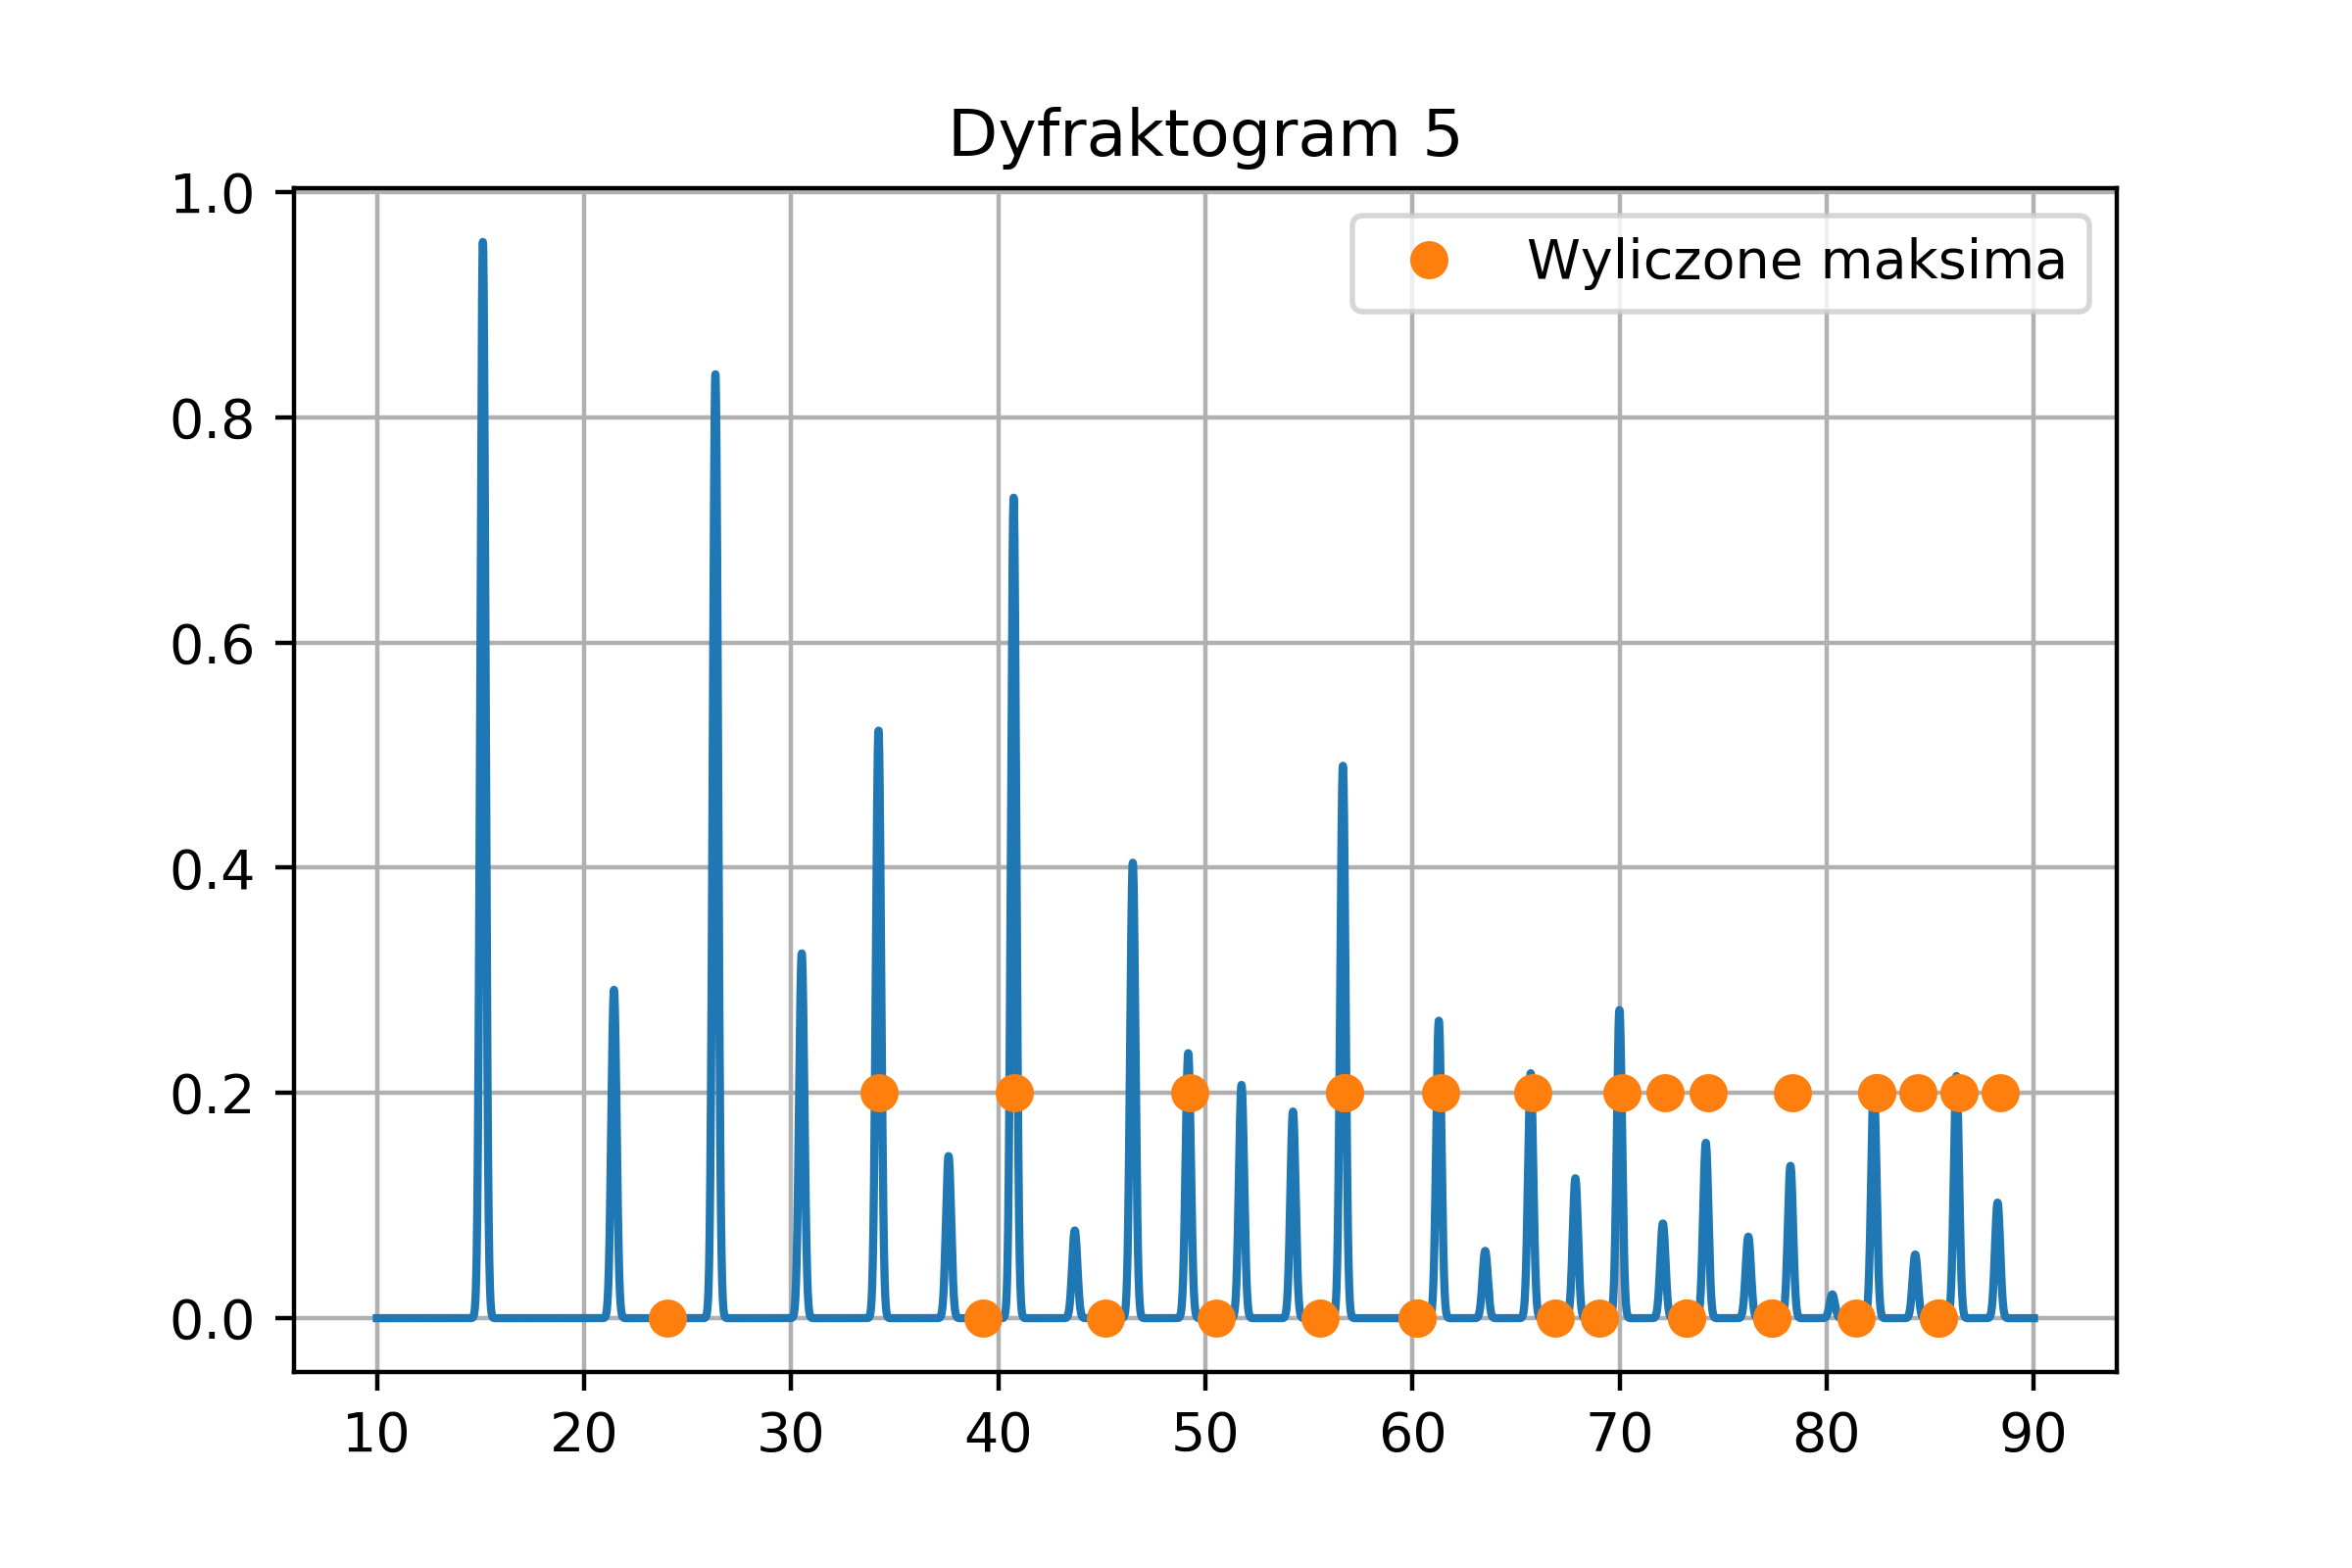
\includegraphics[width=\textwidth]{../Dyfraktogram.png}
\end{figure}

Ze wszystkich danych nam dyfraktogramów ten(5) najlepiej zgadza się z powyższą tabelką. Nie wszystkie zawarte na nim wzmocnienia zostały wyliczone, ale wszystkie wyliczone wzmocnienia są na nim zawarte, zaś żadne z nieprzewidzianych wzmocnień nie występuje w miejscu wyliczonego wygaszenia. 

\section{Zadanie 5: Testy Baterii Li-Ion}
Pojemność grawimetryczną (q) wyliczyłam ze wzoru $q=\frac{tI} {m} $, gdzie t to czas rozładowania, I to prąd (w tym przypadku $I=59.8\mu A$, zaś m to masa próbki (tutaj $m=3.53mg$). Doświadczalna pojemność grawimetryczna jest maksimum pojemności grawimetrycznej na poniższym wykresie czyli 123.72$\frac{mAh}{g}$.
Teoretyczną pojemność grawimetryczną wyznaczyłam ze wzoru użytego na zajęciach czyli $q = \frac{N_A e}{M_{LiFePO_4}}$ co w rezultacie dało wynik 169.89$\frac{mAh}{g}$. Dla takich wartości pojemność doświadczalna stanowi 72.82\% pojemności teoretycznej.

 \begin{figure}[H]
	\centering
		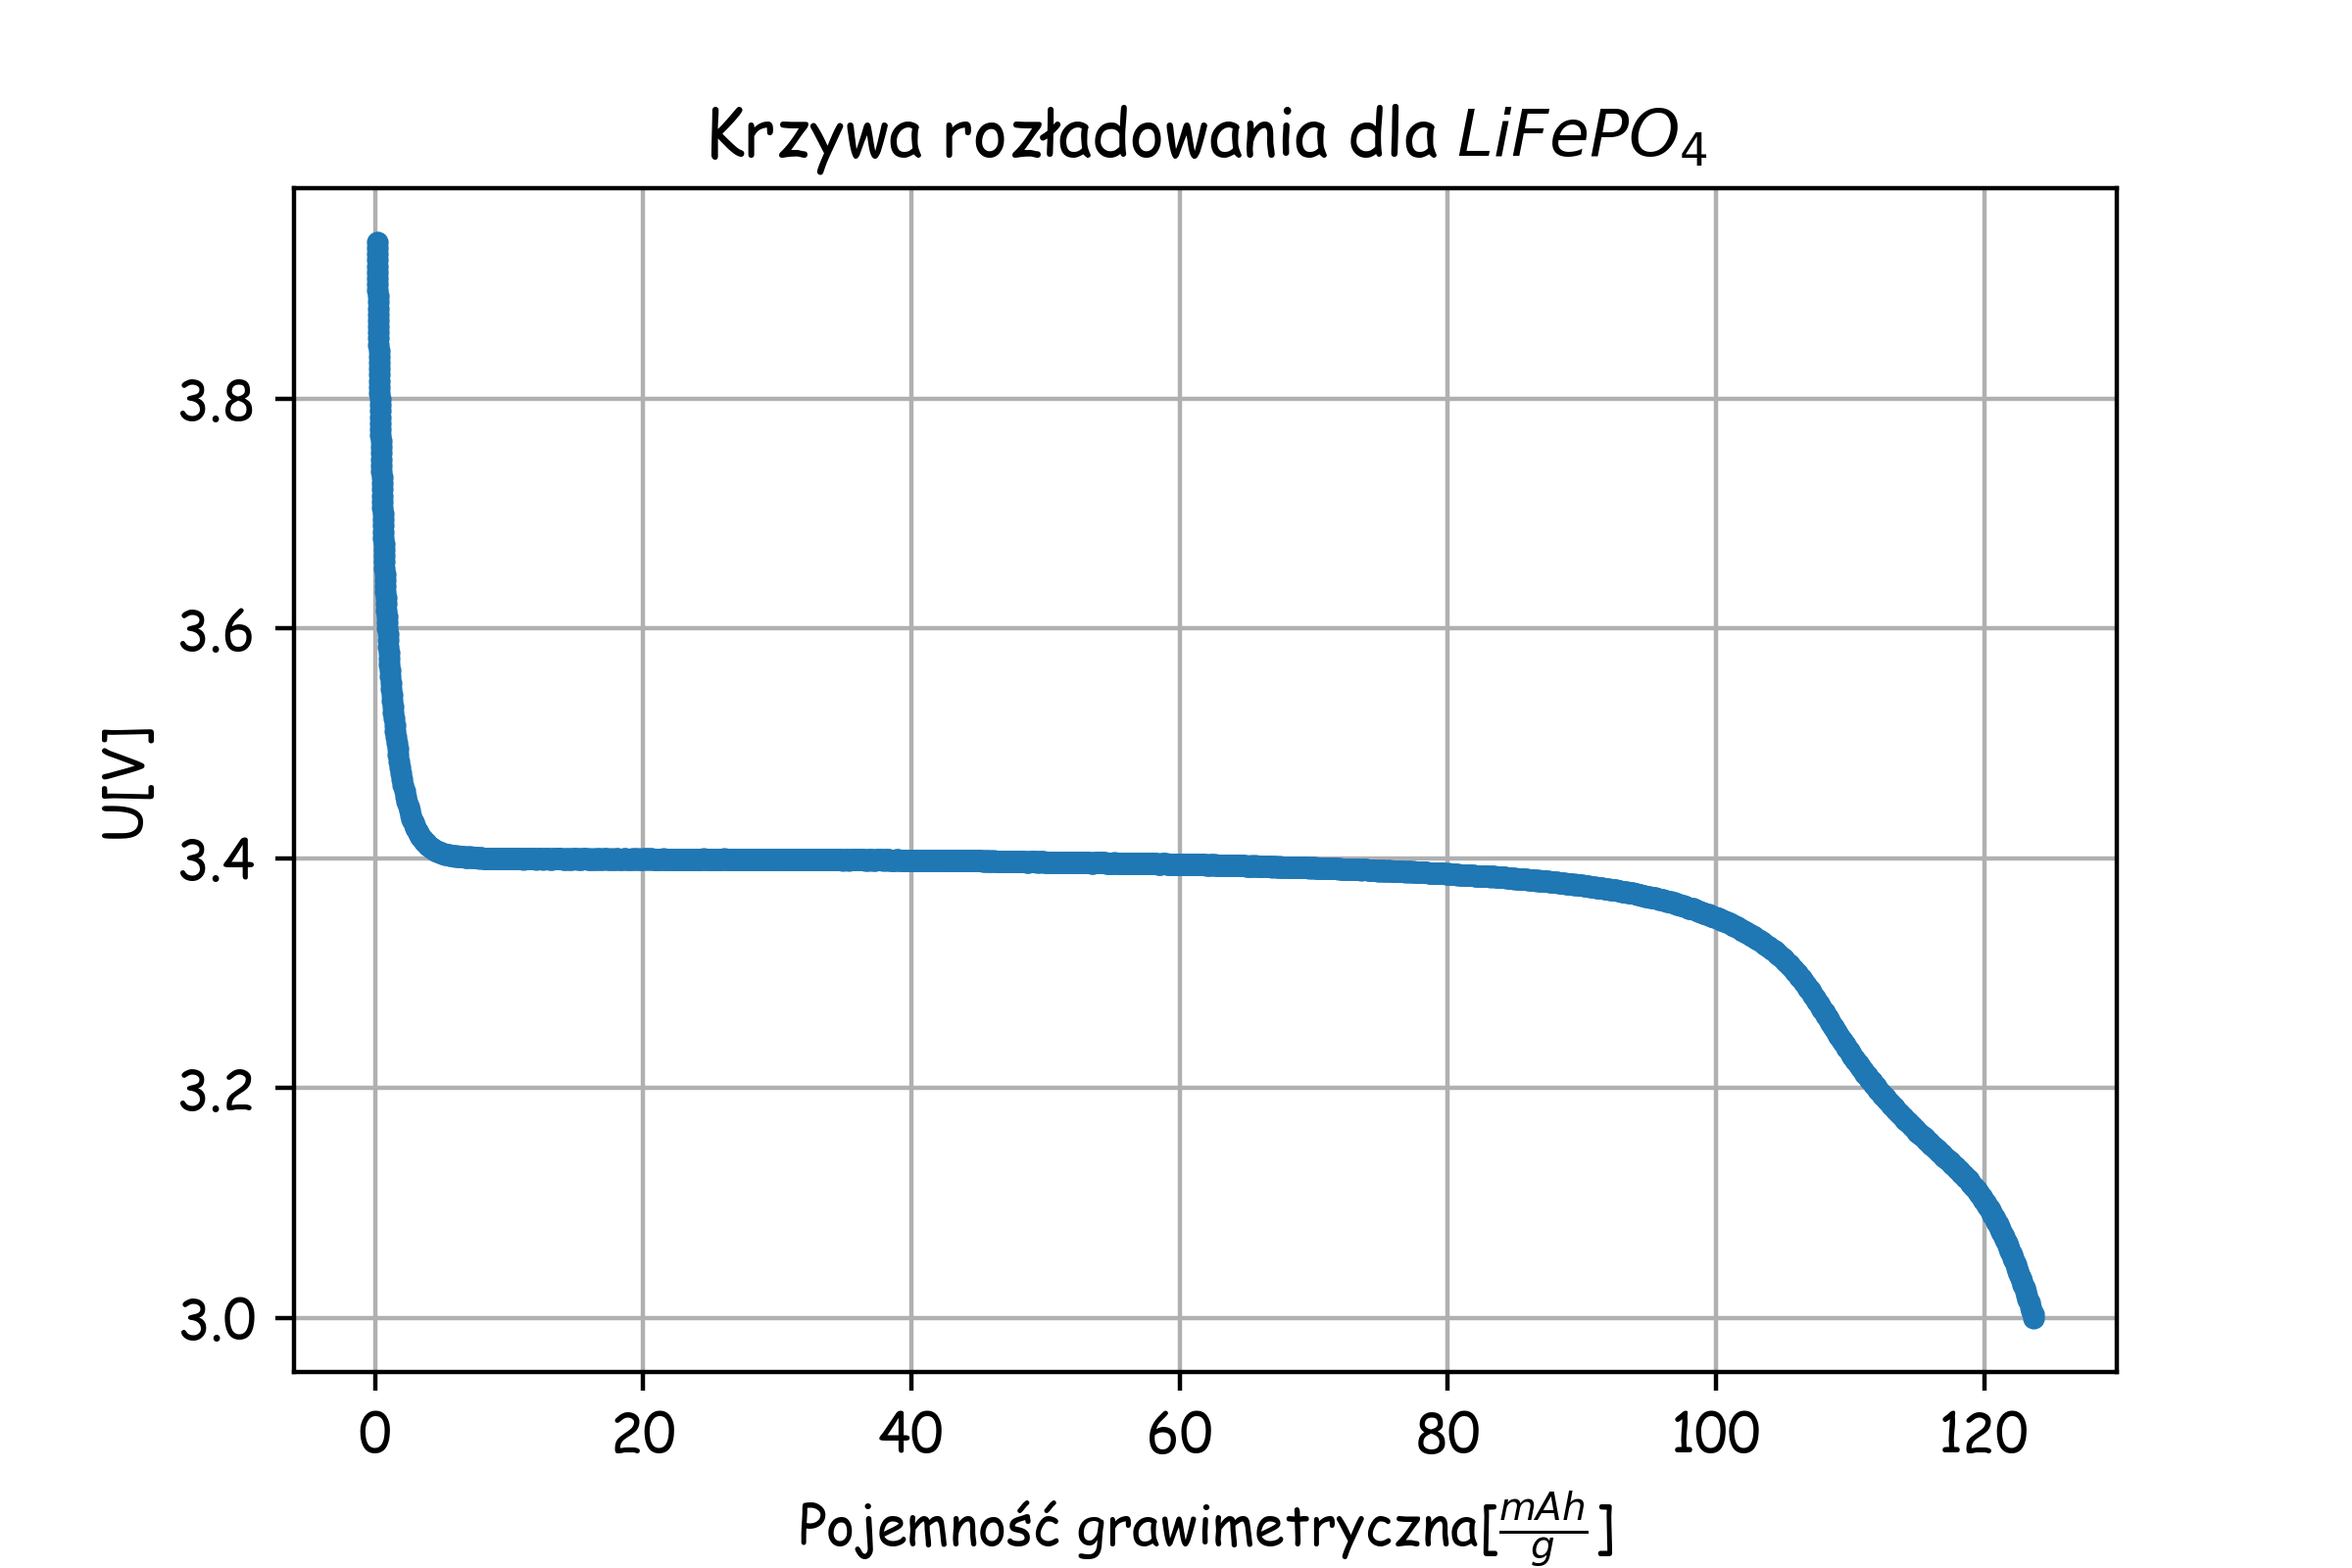
\includegraphics[width=\textwidth]{../Krzywa_rozladowania.png}
\end{figure}

\end{document}
